\documentclass[12pt,a4,xcolor=table]{article}
\usepackage[margin=1in]{geometry}
\usepackage{hyperref}
\usepackage{multicol}
\usepackage{multirow}
\usepackage[table,xcdraw]{xcolor}
\usepackage[rightcaption]{sidecap}
\usepackage{enumitem}
\usepackage{tikz}
\usetikzlibrary{trees}
\usepackage{array,booktabs}
\usepackage{pgfgantt}
\usepackage{rotating}
\usepackage{amssymb}
\usepackage[normalem]{ulem}
\useunder{\uline}{\ul}{}

\title{Literature Review}
\author{}
\date{}

\begin{document}

\begin{titlepage}
	\newcommand{\HRule}{\rule{\linewidth}{0.5mm}}
	\center
	\Large Electronics and Computer Science\\
	\Large Faculty of Physical Sciences and Engineering\\
	\Large University of Southampton\\[1.5cm]
	\Huge Anna Kutseva\\
	{\large 11 December,2018}\\[3cm]
	\HRule \\[0.4cm]
	\textsc{{\huge Exploring Turing Machine Simulations on Social Machines }}\\[0.3cm]
	\HRule \\[1.5cm]
	\LARGE Project supervisor: Thanassis Tiropanis \\
	\LARGE Second examiner: Adam Prugel-Bennett \\[1.5cm]
	\Large A project progress report submitted for the award of BSc Computer Science \\[1.5cm]
\end{titlepage}


\tableofcontents
\thispagestyle{empty}

\newpage
\begin{abstract}
	This project aims to establish a framework around which social machine models can be built and evaluated. Social machines are defined herein as those aggregating input from a number of potentially untrustworthy sources (oracles), be this noisy data or from human input. After review, it appears there are a number of theoretical models built upon standard Turing machines, but as the field is still emerging there is no tool for quickly constructing and testing the efficacy of said machines.
	
	To address this, a plan is constructed to create a reference implementation of the reviewed social machines by building upon an existing tool for modelling Turing machines. These implementations will tuneable based on the properties of the simulated oracles at which point their performance will be compared and evaluated for extension in future work.
\end{abstract}
\thispagestyle{empty}
\clearpage
\pagenumbering{arabic} 

\section{Introduction}
\subsection{Problem}
Large and complex computer systems no longer only involve machines performing deterministic operations; there are cases where human input is an integral part in the completion of a certain task or advancing through a continuous process. With the rise of the World Wide Web people have been prompted to not only interact with each other online, but with systems they can contribute to. Such systems can be classified as social machines, as the dependency of their states on the non-deterministic nature of human participants conveys the interweaving of computer logic with real-life knowledge.
\subsection{Goals}
This project aims at finding a way to simulate such environments, thus evaluating the feasibility of modelling social machine components using Turing machine simulations.
There are three major stages this objective has:
\begin{enumerate}[label=\textit{Stage \arabic*}]
	\item Gather a selection of models and classification frameworks to formally define the different behaviours of each component implementation
	\item Find an appropriate open source Turing Machine simulation framework and extend it with implementations of these extra models
	\item Assess the performance and accuracy of these simulations based on theoretical input scenario data or example data if such is available.
\end{enumerate}
Though largely sequential as each stage depends on the previous, it is acknowledged that there will be some amount of overlap as concepts require clarification or alignment moving forward.

\subsection{Scope}
Following the literature review it would seem that most previous endeavours into the domain have remained purely theoretical and as such evaluation metrics will be relatively basic. There is an intention to contact the wider academic community on this topic, but otherwise this project will focus primarily on the implementation rather than attempting to populate an expansive data set for testing all possible metrics and scenarios moving forward.

\newpage
\section{Literature Review}
\subsection{Turing Machines}
\subsubsection{Concept}
The initial concept of the now famous Turing machine was created as a mechanism to prove that the Entscheidungsproblem is unsolvable \cite{Turing1936} but turned out to have many further applications. While Alan Turing's take of machine learning \cite{Turing1969} %original was from 1948 
and human-like conciousness \cite{Turing1950}, although possible to emulate with state machines, were way ahead of their time, his model of abstract a(utomatic)-machines contributed greatly on the foundations of the computer science field.

\paragraph{Formal definition}\hfill\\

$M=\langle Q,\Gamma ,\Sigma,b,q_{0} ,\delta ,F\rangle$
\cite{Hopcroft1979} where:
\begin{multicols}{2}
	\begin{itemize}
		\item Q - the finite set of states
		\item $\Gamma$ - the complete alphabet set
		\item $\Sigma \subseteq \Gamma \setminus \{b\}$ - the set of tape symbols
		\item $b\in\Gamma$ - the blank symbol
		\item $q_{0}\in Q$ - the start state
		\item $\delta :(Q\setminus F)\times \Gamma \rightarrow Q\times \Gamma -  \times \{L,R\}$ - the transition function
		\item $F\subseteq Q$ - the set of accepting states\footnote{There exist variations of the definitions with regards to accepting and rejecting states, but they are all proven to be equivalent. This one follows the definition taken from 'Introduction to automata theory, languages, and computation'\cite{Hopcroft1979}. In section \ref{sec:omega} single \textit{accept} and \textit{reject} states are used instead, following the 'Introducing the $\Omega$-machine' paper\cite{Zhang2014}}
	\end{itemize}
\end{multicols}

%\subsubsection{Implementation}
%\paragraph{A Turing Machine Simulator}\cite{Curtis1965}
%\subsubsection{Other Turing Machines (informally defined)}
%\paragraph{U-Machines}
%\paragraph{C-Machines}
\subsection{O-machines}
There exists a less known idea for an abstract machine by Turing, which was introduced in his PhD thesis - the \textit{o-machine}. Similarly to a-machines\footnote{The Turing machines that are familiar to the greatest number of people in the field.}, o-machines can be described through tables. The main difference between o-machines and other abstract machines, such as a-machines, is the black box element, called an 'oracle'. The latter's definition in is not expanded on in Turing's paper, beyond being depicted as \textit{"some unspecified means of solving number theoretic problems"}\cite{Turing1938}. No details on the internal configuration of an instance of such a machine are available. The o-machine is equipped with one or more oracles, each of which can perform a primitive operation that returns the values of a non-Turing-machine-computable\footnote{In other words - number theoretic} function\cite{Copeland1998} in the form \[ p:\mathbb{N}\mapsto \mathbf{2} \]

The black box nature of the oracles allows for assumptions about what o-machines could represent. One proposed interpretation is that a human brain can be simulated by an o-machine\cite{Copeland1998}. Within the context of modelling social machines, a set of oracles can be utilised as stand-ins for a group of human individuals. Any taken series of actions in a certain environment can be broken down to a set of decision problems, which will then be emulated by the two-valued functions of the oracles.

\begin{multicols}{2}
	[According to van Melkebeek\cite{Melkebeek}, an o-machine has the following components:]
	\begin{itemize}
		\item Shared with traditional TMs:
		\begin{description}
			\item[work alphabet] a set of symbols which can be written on the work tape
			\item[work tape] an infinite sequence of cells that can either be empty or contain a symbol from the tape alphabet
			\item[read/write head] a component located on a single tape cell at a time that can move left or right on the work tape, as well as read and write\footnote{or delete by placing a 'blank symbol'} symbols on it
			\item[control mechanism] responsible for performing actions such as moving the head, manipulating data and switching states\\\\\\
		\end{description}\columnbreak
		\item Additional components
		\begin{description}
			\item[oracle alphabet] a set of symbols that may or may not be different from the work alphabet
			\item[oracle tape] a semi-infinite tape of cells that can either be empty or contain a symbol from the oracle alphabet
			\item[oracle head] acts the same way as the RW head, but on the oracle tape
			\item[\texttt{ASK} and \texttt{RESPONSE} states] when the oracle enters \texttt{ASK} state, the current oracle tape contents are taken as a problem instance and given as an input to the oracle, which, upon finding the problem solution, replaces the work tape contents with its output; the head is moved to the beginning of the tape; state is set to \texttt{RESPONSE}
		\end{description}
	\end{itemize}
\end{multicols}



%\subparagraph{First mention}


%\subparagraph{Turing's O-machines, Searle, Penrose and the Brain}\cite{Copeland1998}
%\subparagraph{Olympia and other O-machines}\cite{Klein2015}
%\subsection{Beyond Turing Machines?}
%\paragraph{Computation Beyond Turing Machines}\cite{Wegner19933}
\subsection{Interaction}

Machines established solely on the basis of computable functions fall flat in modelling present-day computing, considering its trademarks are \textit{interaction} and \textit{reactivity}\cite{Goldin2004}. Having in mind the notion that interactive systems are more expressive than algorithmic ones\cite{Wegner1997}, we can look into evolving the traditional models into something more applicable to the current technological circumstances. 

The TM component of the project can be modelled like a Persistent Turing Machine, with a work and output tapes\footnote{Possibly an input tape as well, if determined as needed.}.

%\paragraph{Elements of Interaction}\hfil\\
%Talking about concurrent computation\cite{Milner1993}
%\paragraph{Turing machines, transition systems and interactions}\hfill\\
%Persistent Turing Machines - for the o-machines or the main machine or both?\cite{Goldin2004}
%\paragraph{The Turing machine model extended with interaction}\cite{Erkens}

\subsection{Social Machines}
The concept of a social machine revolves around the idea of collaborative problem solving \cite{Luczak-Rosch2015}. As defined by  Tim Berners-Lee, they are \textit{"processes in which the people do the creative work and the machine does the administration"}\cite{berners2001weaving}.

 The combination of predefined machine transitions and probabilistic human input allows for introducing a plethora of outcomes for even a single system if it gets exposed to different selections of people. This is closer to the reality of modern computing, than the strict schemas of Turing machines. \footnote{While non-deterministic counterparts of the latter exist, they are closer in potential to being abstract machines than actual representations of the ever-increasing and practically boundless total of branches each interaction presents in real time.}

By reinforcing connection and collaboration between people, social machines indicate existing relationships among themselves. One type of association they exhibit is belonging to one another and thus having types that can be arranged in a hierarchical tree with the World Wide Web as an infrastructure being its root (See Figure \ref{fig:sm-tree}) \cite{Shadbolt2009}.

\begin{SCfigure}[1][h!]
	\centering
	\tikzstyle{every node}=[draw=black,thick,anchor=west]
	\tikzstyle{selected}=[draw=red,fill=red!30]
	\tikzstyle{optional}=[dashed,fill=gray!50]
	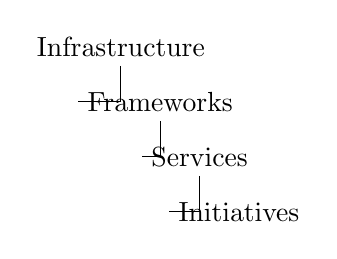
\begin{tikzpicture}[%
	grow via three points={one child at (0.5,-0.7) and
		two children at (0.5,-0.7) and (0.5,-1.4)},
	edge from parent path={(\tikzparentnode.south) |- (\tikzchildnode.west)}]
	\node {Infrastructure}
	child { node {Frameworks}
		child { node {Services}
			child { node {Initiatives}
			}
		}
	};
	\end{tikzpicture}
	\caption{Granularity levels of social machines - \textit{Initiatives} (a.k.a. \textit{Projects}) using \textit{Services} built upon \textit{Frameworks} contained into the Infrastructure}
	\label{fig:sm-tree}
\end{SCfigure}

\paragraph{The emerging web of social machines}
Studies the relationships between SMs\cite{Silvio2010}
\paragraph{From the semantic web to social machines: a research challenge for AI on the World Wide Web}
Connects the semantic web with SMs and provides future goals\cite{Hendler2009}

\subsubsection{Social Machine and Computation Examples}
Given a lack of evaluation data found during the literature review, a few real-world social machines have been identified with the possibility of simulation by reducing the domain and action set of the oracles and machine respectively to a few representative outcomes (both positive and negative):
\paragraph{Wikipedia}
Serving as one of the most well-known cases of social machines, Wikipedia would not exist without the endless flow of human input. It confirms the capacity of social computation by being the largest encyclopedia in existence, that is being updated at such a rate that physically publishing its content is absolutely redundant. Unfortunately, it is speculated that Wikipedia has recently been in decline\cite{simonite2013decline}. A correct simulation of the lifetime of a similar (and preferably simplified) online collaborative knowledge project could predict tendencies in increases and declines of activity
\paragraph{Games with a Purpose}
It is beyond doubt that gamification is a powerful motivation method - simply adding a score number next to a person's username sparks the desire to increase said number. As such, it can be used to encourage meaningful contributions to a real-world broad scope problems through an entertainment platform \cite{Ahn2006}. However, this genre of games is far from being as popular as other genres. The few notable examples that have been used to justify the importance and efficacy of GWAPs\cite{von2008designing} are as of today defunct. Carrying out simulations of such games during their development may demonstrate potential issues, whose resolution may lead to the games' longer life and higher recognition.

\paragraph{The DARPA Network Challenge}

The DARPA Network Challenge The Defense Advanced Research Projects Agency organises annual prized challenges to stimulate problem solving through group effort in search of revolutionary research approaches. In 2009 DARPA presented the efficiency of social computation and crowdsourcing with the following challenge: ten weather balloons were scattered across the United States and had to be located in the shortest time possible. The participating teams used various forms of social networking to achieve their goal, and the winning team managed to complete the task in just 9 hours by putting a referral system and cash incentives to use. Many of the strategies were essentially incorporating social computation to tackle the problem in a much faster way by engaging people, rather than by setting up a massive fully automated detection system\cite{Robertson2013}. As several of the winning strategies are publicly shared\cite{tang2011reflecting}, they could potentially be simulated and compared given differing oracle behaviours as part of this project.

\section{Work Completed}
\subsection{Desing and Implementation}
\subsubsection{The Omega Machine}\label{sec:omega}
The proposed implementation of a social machine model is the $\Omega$-machine, that serves as an extended model of the Turing machine, employing o-machines whose oracles act as human individuals\cite{Zhang2014}. The initial configuration based on the omega-machine idea is:
\[\langle Q, \Sigma, \Gamma, \delta, q_{0}, q_{accept}, q_{reject},\Gamma_{\omega} ,\delta_{\omega}\rangle\] 
where $\Gamma_{\omega}$ is the oracle alphabet and $\delta_{\omega}$ is the transformation function for the oracles. Upon creation, each oracle belonging to a certain omega-machine instance will only need to have its \texttt{ASK} and \texttt{RESPONSE} states be specified. In this case: \[\langle M, s_{ASK}, s_{RESPONSE} \rangle\] where M is the omega-machine that the oracle belongs to and from which it \textit{inherits} the oracle alphabet and the transformation function. The first version of the social machine model will be built following this structure.

If time allows, the the $\delta_{\omega}$ component may be broadened into $\Delta_{\omega}$, which would support a different function for each oracle instance, looking like: \[\langle M, \delta_{\omega}, s_{ASK}, s_{RESPONSE} \rangle\] where $\delta_{\omega} \in \Delta_{\omega}$, meaning there is a variety of functions that could be assigned to the oracle from a predefined whitelist, and the a machine would be modified into: \[\langle Q, \Sigma, \Gamma, \delta, q_{0}, q_{accept}, q_{reject},\Gamma_{\omega} ,\Delta_{\omega}\rangle\]

In this way the oracle cluster part of the model can come closer to resembling a crowd of diverse individuals.

Ideally, the ultimate configuration goal would be to have o-machines be as independent from the core a-machine as possible:
\[M = \langle Q, \Sigma, \Gamma, \delta, q_{0}, q_{accept}, q_{reject},\rangle\]
\[O = \langle M, \Gamma_{\omega}, \delta_{\omega}, s_{ASK}, s_{RESPONSE} \rangle\]
where the o-machine has a reference to the a-machine, but the a-machine does not have a reference to any of the o-machines, mimicking the behaviour of a system, which is logically independent from the specific properties of its users. Conclusively, a social machine, or an omega-machine will then be defined as \[\Omega = \langle M, \mathbb{O} \rangle \] where M represents the technical platform, or the \textit{machine} part, and $\mathbb{O}$ represents the set of oracles, or the \textit{social} part.


\subsection{Open Source Analysis}

\subsubsection{Criteria}
Deciding on a framework to extend is a virtually irreversible(See Table \ref{table:risk3} in Appendix \ref{sec:app}) and as such should be considered strongly before making a decision. The web contains a myriad of open source software options, most of which can be found on websites such as \texttt{sourceforge.net}. Notwithstanding, many, if not most, of those projects lack support, reviews, and proper documentation, which marks them as unsound options. To support the final choice, each option was evaluated against the following list of criteria:
\begin{description}
	\item[Acclaim] A well recognised, favourably reviewed piece of software promises a good groundwork for the experiment and increases the likelihood of it being built upon in future work.\\
			\underline{Questions to ask:} \textit{Is there any academic or industrial usage? Is the overall feedback thorough and positive?}
	\item[Language] Implementation in a modern and widely utilised language ensures quick uptake.\\
			\underline{Questions to ask:} \textit{What language is it written in? Is the language an adequate choice for the task? Am I familiar with this language? }
	\item[Maintenance] Proper and frequent support promises fewer performance issues and bugs. Also, large involvement with the project indicates large amount of effort, and consequently - good quality of the product.\\
			\underline{Questions to ask:} \textit{What are the activity levels on any associated forums or code repositories? How often have past updates been rolled out? When was the most recent update?}
	\item[Functionality] A large code-base reduces the need to implement basic or common features.\\
			\underline{Questions to ask:} \textit{Is the program expressive enough to be extended efficiently? Are there components I can reuse in multiple ways?}
	\item[Documentation] Well commented code will be easier to work with; any additional instructive materials, such as help pages, example tutorials, readme files, or full manual documents provide evidence of usability and accessibility; thorough change logs give more insight on development, and further inform about handled or potential issues.\\
			\underline{Questions to ask:} \textit{Is it well commented? Is there a dedicated website, user manual, or a readme file? Are there any examples or tutorials? Is there a comprehensive change log for recent updates?}
\end{description}

\subsubsection{Options}
Below is a selection of eight contenders that were considered.

\begin{multicols}{4}
	\paragraph{JFLAP} 
	Educational software by the Duke University, written in Java. It has been around since 1996 but it is still being updated - the latest release is from 2018 and running on Java 8. The program creator Susan Rodger has been recognised in the academic field as an ACM Distinguished Member, and awarded the ACM Karl V. Karlstrom Outstanding Educator Award. Beside Turing machines, JFLAP enables simulations for numerous other topics on automata and formal languages. The user interface is done using Java Swing.
	%\columnbreak
	\paragraph{Tursi}
	Created in Java by the German developer Claus Schätzle. It can be used both through a GUI or in a console. It works with specifically designed .tm files for the system written in a Turing machine based language. Its distinctive features include exporting tables to state diagrams, history and break states.
	%\columnbreak
	\paragraph{Owen's Turing \\Machine Simulator}
	A Turing Machine simulator, developed  in Java by Owen Kellett. It uses files with a .tmo extension. Its user interface is also built with Java Swing.
	%\columnbreak
	\paragraph{Tuatara} 
	Written in Java Swing, last updated in 2007. It has a simple point-and-click interface. Out of the selection found in SourceForge it was the only project with recent downloads, as well as a review. 	
	%\columnbreak
	\paragraph{TMSimulator}
	The only application to use JavaFX instead of Swing. A student project from the technical university of Vienna. Last updated in 2011.
	%\columnbreak	
	\paragraph{JSTuring}
	Web-based simulator in JavaScript. It uses .txt files for processing machines. The last commit was made in June 2018.
	%\columnbreak
	\paragraph{Tm}
	HTML based with sample machines that are hard-coded.
	
	\paragraph{TuringSym}
	Written in Delphi. Last modified in 2004.
	
	
\end{multicols}

\subsubsection{Choice}

The majority of open source projects available are implemented in Java and have user interfaces built with the Swing toolkit. After inspecting the source code contents and considering factors such as support, functionality, public feedback and quality of documentation, I strongly decided in favour of JFLAP \cite{rodger2006jflap}, as it excelled in all the aforementioned requirements in comparison to the rest of the projects. In fact, its diverse functionality and multitude of classes for any sub-entity that might be needed will enable easier and cleaner implementation of the social machine model.


\section{Plan of Remaining Work}

\subsection{Timeline}

With the bulk of the literature review complete below is outlined the timeline for the remaining work as part of this project (see Figure \ref{fig:gantt} in Appendix \ref{sec:app}). Having decided on JFLAP as the framework of choice, the majority of the upcoming weeks will be spent on design and implementation of the various models identified in the literature review, based on the structure and available components within JFLAP. As this is the centrepiece product of the project, unfortunately this cannot be broken down to run in parallel with any other tasks except for testing once implementation nears completion. After implementation, the various models will be compared and evaluated based on metrics that are yet to be identified at this point and conclusions can be drawn as the tests are run.

Alongside the consideration for concurrently executable tasks, extra time has also been set aside for known and unknown interruptions. Most notably are the blocks of time dedicated to the more intense study periods surrounding exams and the weeks during the holidays where inability to progress due to family engagements are highly likely. Particularly the Christmas period has been set aside  for recovery before the next term begins. Although the Easter break has also been marked as a holiday for planning purposes, its proximity to the final deadline suggests that a certain amount of work will need to be done in this period as well. Finally all expected task durations have been overestimated by roughly 20\% to accommodate for unforeseen events and general delays. With this in mind, ideal progress should be ahead of the Gantt chart estimation and falling behind would be an indication of some underlying time management or complexity issue.

\subsection{Risk Analysis}

To complement the timeline breakdown of upcoming work, a risk analysis has been performed to anticipate potential issues that would have a significant impact on the project's progress. Each risk was assigned a Likelihood (L) and Severity (S) which multiply together to produce the overall Risk score colour coded by concern (see Tables  \ref{table:risk1}, \ref{table:risk2} and \ref{table:risk3} in Appendix \ref{sec:app}). Once classified, mitigation strategies and contingency plans were assigned in an attempt to address the concerns ahead of time and help factor in any recovery period into the timeline assessment. Concluding from this analysis, issues arising during implementation accompanied the highest risk factor and as such have been granted the largest allocation of time in the Gantt chart.

\newpage
\appendix
\section{Appendix}
\label{sec:app}

\begin{table}[h!]
	\centering
	\caption{Management Issues}
		\label{table:risk1}
\footnotesize
\begin{tabular}{|>{\centering}m{1.5in} |>{\centering}m{0.1in} |>{\centering}m{0.1in} |>{\centering}m{0.3in} |>{\centering}m{1.8in} |>{\centering\arraybackslash}m{1.8in}|}
	\hline
	\textbf{Problem}                                                 & \textbf{L}                & \textbf{S}                  & \textbf{Risk}                      & \textbf{Mitigation}                                                                                                                                               & \textbf{Contingency}                                                                                                                                                                 \\ \hline
	Falling behind schedule due to clashes with other assessed tasks & \cellcolor[HTML]{FFC702}\textit{3} & \cellcolor[HTML]{FFC702}\textit{3} & \cellcolor[HTML]{FFC702}\textbf{9} & Extra time allocated for the period surrounding exams. One hour of work allocated per day as a minimum in parallel with other modules.                            & Identify problem modules and assessments as early as possible to raise with supervisor ASAP.                                                                                         \\ \hline
	Falling behind schedule due to slow progress                     & \cellcolor[HTML]{F8FF00}\textit{2} & \cellcolor[HTML]{FFC702}\textit{3} & \cellcolor[HTML]{FFC702}\textbf{6} & Tasks defined requiring more time than estimated by default to act as an on-going buffer. Burn-down chart to be kept up-to-date for sub-goals across entire year. & Actual work should ideally run ahead of the Gantt chart given the extra time included. If falling behind then remaining work and Gantt chart should be re-evaluated with supervisor. \\ \hline
	Unavailability of supervisor                                     & \cellcolor[HTML]{ABCB00}\textit{1} & \cellcolor[HTML]{FFC702}\textit{3} & \cellcolor[HTML]{F8FF00}\textbf{3} & Maintain attendance of weekly supervisor meetings. Prepare multiple tasks to carry out ahead of time in case a meeting has to be skipped.                         & Continue with tasks as planned, maintain contact with supervisor by any means available. Contact university for support in extreme case of extended absence.                         \\ \hline
	Licensing issues                                                 & \cellcolor[HTML]{ABCB00}\textit{1} & \cellcolor[HTML]{F8FF00}\textit{2} & \cellcolor[HTML]{F8FF00}\textbf{2} & Utilise open-source software, ideally that which has already been attributed by other academic use-cases. Contact authors for permission.                         & Comply with author's requests. Publish products of project as permissible under appropriate license with referencing as necessary.                                                   \\ \hline
	Illness                                                          & \cellcolor[HTML]{F8FF00}\textit{2} & \cellcolor[HTML]{F8FF00}\textit{2} & \cellcolor[HTML]{F8FF00}\textbf{4} & Extra time buffer can be used for sick days as necessary.                                                                                                         & Re-evaluate remaining tasks as appropriate.Contact supervisor and university to advise in extreme cases.                                                                             \\ \hline
\end{tabular}
\end{table}

\begin{table}[h!]
	\centering
	\caption{Technical Issues}
	\label{table:risk2}
	\footnotesize
	\begin{tabular}{|>{\centering}m{1.5in} |>{\centering}m{0.1in} |>{\centering}m{0.1in} |>{\centering}m{0.3in} |>{\centering}m{1.8in} |>{\centering\arraybackslash}m{1.8in}|}
		\hline
		\textbf{Problem}              & \textbf{L}                         & \textbf{S}                         & \textbf{R}                         & \textbf{Mitigation}                                                                                          & \textbf{Contingency}                                         \\ \hline
		Hardware not powerful enough  & \cellcolor[HTML]{F8FF00}\textit{2} & \cellcolor[HTML]{F8FF00}\textit{2} & \cellcolor[HTML]{F8FF00}\textbf{4} & Design model components with performance in mind. Utilising university hardware as necessary.                & Contact supervisor to request access to specialist hardware. \\ \hline
		Damaged hardware              & \cellcolor[HTML]{ABCB00}\textit{1} & \cellcolor[HTML]{ABCB00}\textit{1} & \cellcolor[HTML]{ABCB00}\textbf{1} & Ensure program and development environment are accessible from multiple sources (not just personal machine). & Utilise university hardware.                                 \\ \hline
		Loss of work (code or report) & \cellcolor[HTML]{ABCB00}\textit{1} & \cellcolor[HTML]{FFC702}\textit{3} & \cellcolor[HTML]{F8FF00}\textbf{3} & Frequent back-ups to local drives and commits to remote repositories.                                        & Retrieve latest copy from backup.                            \\ \hline
	\end{tabular}
\end{table}

\begin{table}[h!]
	\centering
	\caption{Implementation Issues}
	\label{table:risk3}
	\footnotesize
	\begin{tabular}{|>{\centering}m{1.5in} |>{\centering}m{0.1in} |>{\centering}m{0.1in} |>{\centering}m{0.3in} |>{\centering}m{1.8in} |>{\centering\arraybackslash}m{1.8in}|}
		\hline
		\textbf{Problem}                                               & \textbf{L}                                                & \textbf{S}                                                & \textbf{R}                          & \textbf{Mitigation}                                                                                                  & \textbf{Contingency}                                                                                          \\ \hline
		Chosen framework is not appropriate for implementing the model & \cellcolor[HTML]{F8FF00}\textit{2}                        & \cellcolor[HTML]{F88602}{\color[HTML]{333333} \textit{4}} & \cellcolor[HTML]{FFC702}\textbf{8}  & Appropriate analysis made before framework selection.                                                                & Implement closest approxiamation using next most appropriate tooling. Document findings regardless.           \\ \hline
		Difficulty grasping important concepts                         & \cellcolor[HTML]{F8FF00}\textit{2}                        & \cellcolor[HTML]{F8FF00}\textit{2}                        & \cellcolor[HTML]{F8FF00}\textbf{4}  & Extensive literature review before beginning implementation. Regular contact with supervisor and academic community. & Schedule additional meetings with supervisor focussed on specific topics as soon as possible to avoid delays. \\ \hline
		Insufficient methods of evaluation                             & \cellcolor[HTML]{F88602}{\color[HTML]{333333} \textit{4}} & \cellcolor[HTML]{FFC702}\textit{3}                        & \cellcolor[HTML]{F88602}\textbf{12} & Contact academic community and review any evaluation performed in available literature.                              & Discuss potential metrics with supervisor and evaluate to best of ability.                                    \\ \hline
		High algorithmic complexity                                    & \cellcolor[HTML]{F8FF00}\textit{2}                        & \cellcolor[HTML]{FFC702}\textit{3}                        & \cellcolor[HTML]{FFC702}\textbf{6}  & Review and optimise code as implemented to minimise overhead on top of underlying algorithmic complexity.            & Request access to specialist hardware to accommodate load.                                                    \\ \hline
		Poorly designed model                                          & \cellcolor[HTML]{F8FF00}\textit{2}                        & \cellcolor[HTML]{FFC702}\textit{3}                        & \cellcolor[HTML]{FFC702}\textbf{6}  & Review code with supervisor during implementation, test as soon as is feasible.                                      & Begin testing and evaluation phases as soon as possible to avoid issues with write-up due to missing data.    \\ \hline
		Bugs                                                           & \cellcolor[HTML]{F88602}{\color[HTML]{333333} \textit{4}} & \cellcolor[HTML]{F8FF00}\textit{2}                        & \cellcolor[HTML]{FFC702}\textbf{8}  & Utilise functionality tests to ensure correctness as soon as possible.                                               & Prioritise evaluation of correct work. Address issues as timing permits.                                      \\ \hline	
	\end{tabular}
\end{table}

\newpage
\begin{sidewaysfigure}[]
	\centering
	\caption[Gantt chart]{Project Gantt chart.}
	\begin{ganttchart}[
		hgrid,
		vgrid={*{6}{draw=none},dotted},
		x unit=0.85mm,
		time slot format=isodate,
		vrule/.style={thick, red},
		milestone right shift = 1,
		milestone left shift = -1,
		newline shortcut=true,
		today=2018-12-11,
		progress=today
		]{2018-10-01}{2019-05-20}
		
		\gantttitlecalendar{year, month=name} \\
		
		\ganttmilestone{Initial meeting}{2018-10-08} \\
		
		\ganttgroup[group label node/.append style={align=right}]{Definition}{2018-10-08}{2018-12-23} \\
		\ganttbar[bar label node/.append style={align=right}]{Project\ganttalignnewline outline}{2018-10-08}{2018-10-11} \\
		\ganttbar[bar label node/.append style={align=right}]{Literature\ganttalignnewline research}{2018-10-15}{2018-12-08} \\
		\ganttbar[bar label node/.append style={align=right}]{Designing\ganttalignnewline the model}{2018-12-01}{2018-12-23} \\
		
		\ganttgroup[group label node/.append style={align=right}]{Implementation}{2018-11-12}{2019-02-28} \\
		\ganttbar[bar label node/.append style={align=right}]{Choosing\ganttalignnewline software}{2018-11-12}{2018-12-01} \\
		\ganttbar[bar label node/.append style={align=right}]{Familiarising with\ganttalignnewline chosen software}{2018-12-03}{2018-12-13} \\
		\ganttbar[bar label node/.append style={align=right}]{Implementation\ganttalignnewline of the model}{2018-12-14}{2019-02-28} \\	
		
		\ganttgroup[group label node/.append style={align=right}]{Evaluation}{2019-02-15}{2019-04-23} \\
		\ganttbar[bar label node/.append style={align=right}]{Functionality\ganttalignnewline testing}{2019-02-15}{2019-03-18} \\
		\ganttbar[bar label node/.append style={align=right}]{Optimisation}{2019-03-01}{2019-04-04} \\	
		\ganttbar[bar label node/.append style={align=right}]{Final\ganttalignnewline evaluation}{2019-03-18}{2019-04-23} \\	
		
		\ganttmilestone{Completed}{2019-04-24} \\
		
		\ganttbar[bar label node/.append style={align=right}]{Preparation\ganttalignnewline for the viva}{2019-04-25}{2019-05-15} \\
		
		\ganttmilestone{Presented}{2019-05-17} 
		
		\ganttvrule[vrule label node/.append style={align=center}]{\ganttalignnewline Brief deadline}{2018-10-12}
		\ganttvrule[vrule label node/.append style={align=center}]{\ganttalignnewline\ganttalignnewline Interim deadline}{2018-12-11}
		\ganttvrule[vrule label node/.append style={align=center}]{\ganttalignnewline Final\ganttalignnewline deadline}{2019-04-30}
		\ganttvrule[vrule label node/.append style={align=center}]{\ganttalignnewline Viva}{2019-05-16}
		\ganttvrule[vrule/.append style={blue, thin}]{}{2019-01-27}
		
		\ganttvrule[vrule/.append style={green, dotted}]{}{2018-12-24}
		\ganttvrule[vrule/.append style={green, dotted}]{}{2018-12-25}
		\ganttvrule[vrule/.append style={green, dotted}]{}{2018-12-26}
		\ganttvrule[vrule/.append style={green, dotted}]{}{2018-12-27}
		\ganttvrule[vrule/.append style={green, dotted}]{}{2018-12-28}
		\ganttvrule[vrule/.append style={green, dotted}]{}{2018-12-29}
		\ganttvrule[vrule/.append style={green, dotted}]{}{2018-12-30}
		\ganttvrule[vrule/.append style={green, dotted}]{}{2018-12-30}
		\ganttvrule[vrule/.append style={green, dotted}]{}{2019-01-01}
		\ganttvrule[vrule/.append style={green, dotted}]{Holidays}{2019-01-02}
		
		\ganttvrule[vrule/.append style={orange, dotted}]{}{2019-01-19}
		\ganttvrule[vrule/.append style={orange, dotted}]{}{2019-01-20}
		\ganttvrule[vrule/.append style={orange, dotted}]{}{2019-01-21}
		\ganttvrule[vrule/.append style={orange, dotted}]{}{2019-01-22}
		\ganttvrule[vrule/.append style={orange, dotted}]{Exams}{2019-01-23}
		
		\ganttvrule[vrule/.append style={green, dotted}]{}{2019-04-01}
		\ganttvrule[vrule/.append style={green, dotted}]{}{2019-04-02}
		\ganttvrule[vrule/.append style={green, dotted}]{}{2019-04-03}
		\ganttvrule[vrule/.append style={green, dotted}]{}{2019-04-04}
		\ganttvrule[vrule/.append style={green, dotted}]{}{2019-04-05}
		\ganttvrule[vrule/.append style={green, dotted}]{}{2019-04-06}
		\ganttvrule[vrule/.append style={green, dotted}]{Holidays}{2019-04-07}
		
		\ganttlink{elem2}{elem3}
		\ganttlink{elem3}{elem4}
		\ganttlink{elem6}{elem7}
		\ganttlink{elem7}{elem8}
	\end{ganttchart}

	\label{fig:gantt}
\end{sidewaysfigure}

\clearpage
\newpage
\bibliographystyle{ieeetr}%needed?
\footnotesize
\bibliography{bib}%\thispagestyle{empty}
\end{document}
